\chapter{Tidyverse}
\section{Z-score scatter plots}

In this exercise we have a data of children between the 0 and 5 years in Kenya with the Z-score for stunting. In the first part we examine the development over time and based on gender of the children. And then based on whether they are living in rural or urban regions.

\begin{itemize}
    \item Using the functions and methods provided by the \textbf{tidyverse} package we can do following tasks;
    \begin{itemize}
        \item data loading
        \item dropping irrelevant variables
        \item checking the type of the remaining variables. 
    \end{itemize}
    \item Using the \textbf{haven} package the data in STATA format is loaded. 
\end{itemize}

\nonumber
After data preparation we plot the age of children against the Z-score.% (variable \texttt{zstunt}).


\begin{itemize}
    \item In the first plot we consider the whole population (see Figure \ref{fig:scatter})
    \begin{enumerate}
        \item We observe that the Z-score decreases after birth from an average level until it nearly reaches the critical threshold of $-2$ at an age about $18$ months. 
        \item After the age of $18$ months the score increases slightly and seems to converge to a limit between $1$ and $-1.5$.
        \item Therefore we observe that children in Kenyan are general are born with an average height.
        \item But, at least until the age of $5$ years children's height is below the average .
        \item It's also important to note that, there is a substantial amount of points below the critical value which suggests that many children considered as stunted.
    \end{enumerate}
\end{itemize}
\begin{figure}[h]
    \centering
		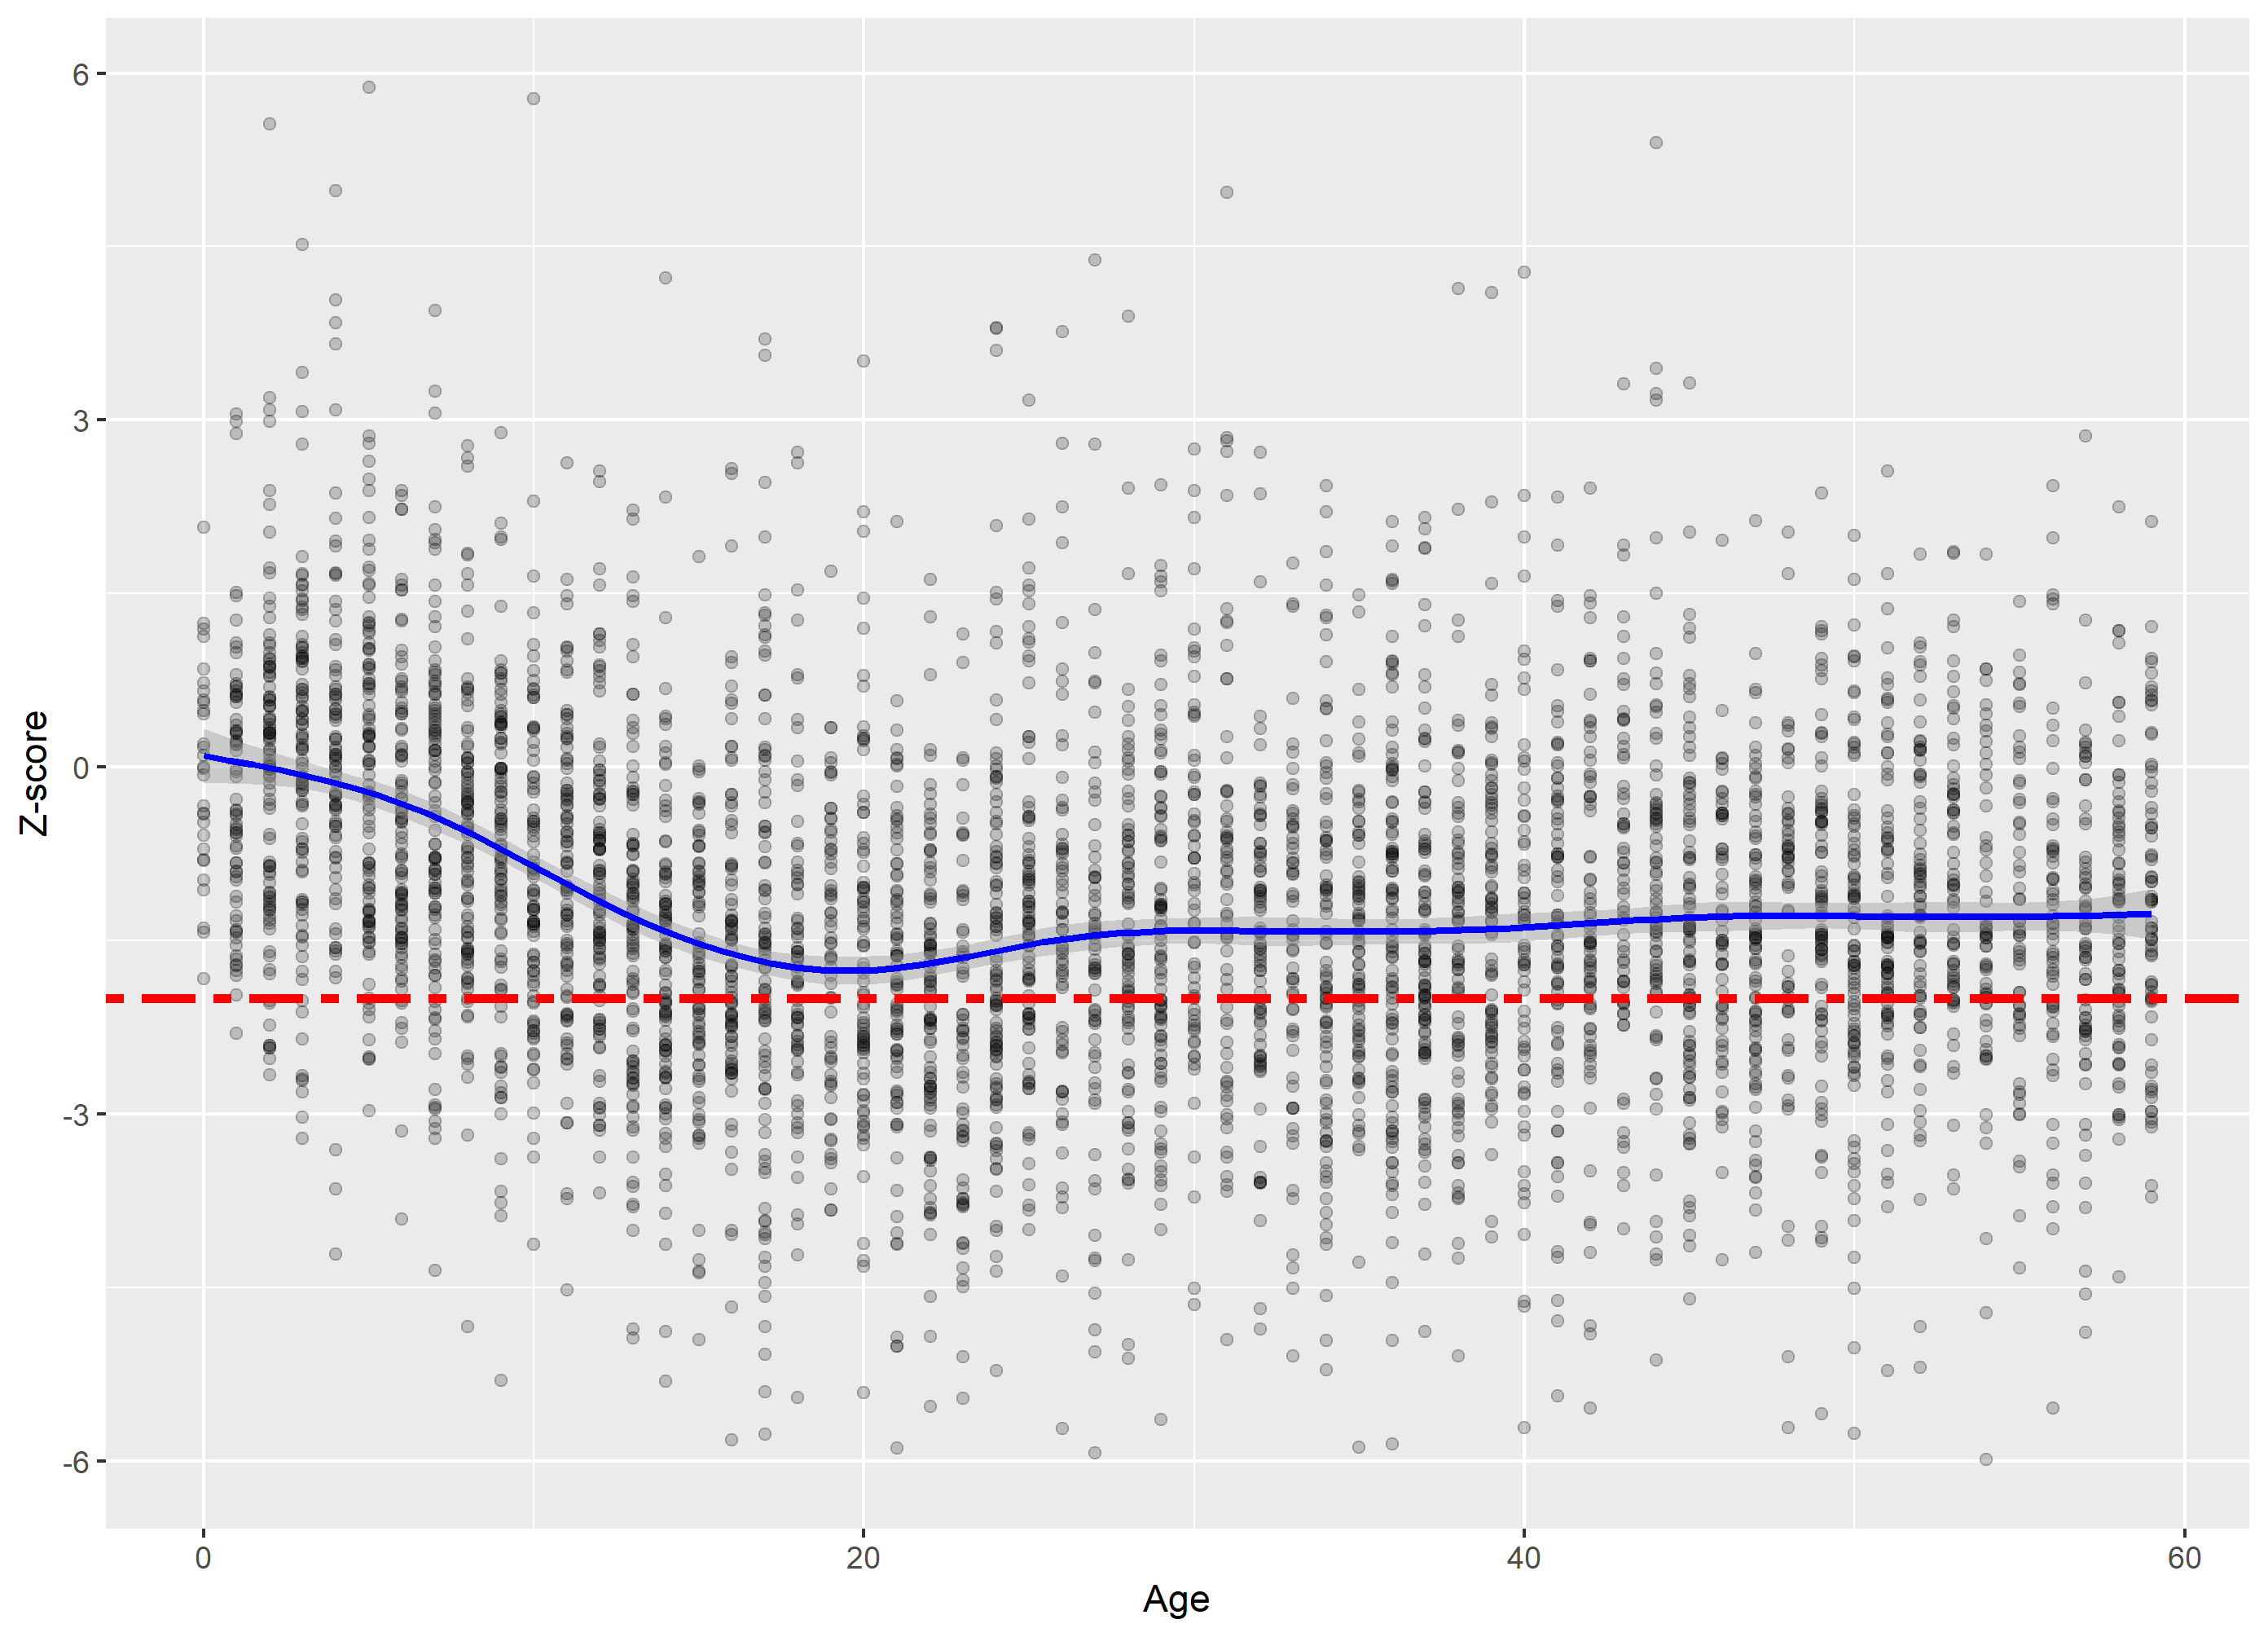
\includegraphics[scale=0.5]{ex1/scatter.png}
		\caption{Scatter plot for age (in months) against Z-score, with a smooth line. The red line (at \texttt{zstunt} $= - 2$) shows the critical value.}
		\label{fig:scatter}
\end{figure}

\newpage
\begin{itemize}
    \item We split the data first based on gender and then based on whether children are living in rural or urban regions of the country. (see Figure \ref{fig:scatter_1})
    \begin{enumerate}
        \item We observe similar patter as we observed for the overall data
        \item We can also observe a slight but visible difference that the Z-score is lower in male children and those who live in rural areas of the country
        \item The difference between the genders in Z-score reduces with time
        \item The inequality caused by the environment seems to persist
        \item We see that for the urban part of the population the Z-score is increasing slowing and approaching an average level
        \item For the children living in rural areas the Z-score seems constant at a value of $-1.5.$
    \end{enumerate}
\end{itemize}

\begin{figure}[h]
    \centering
		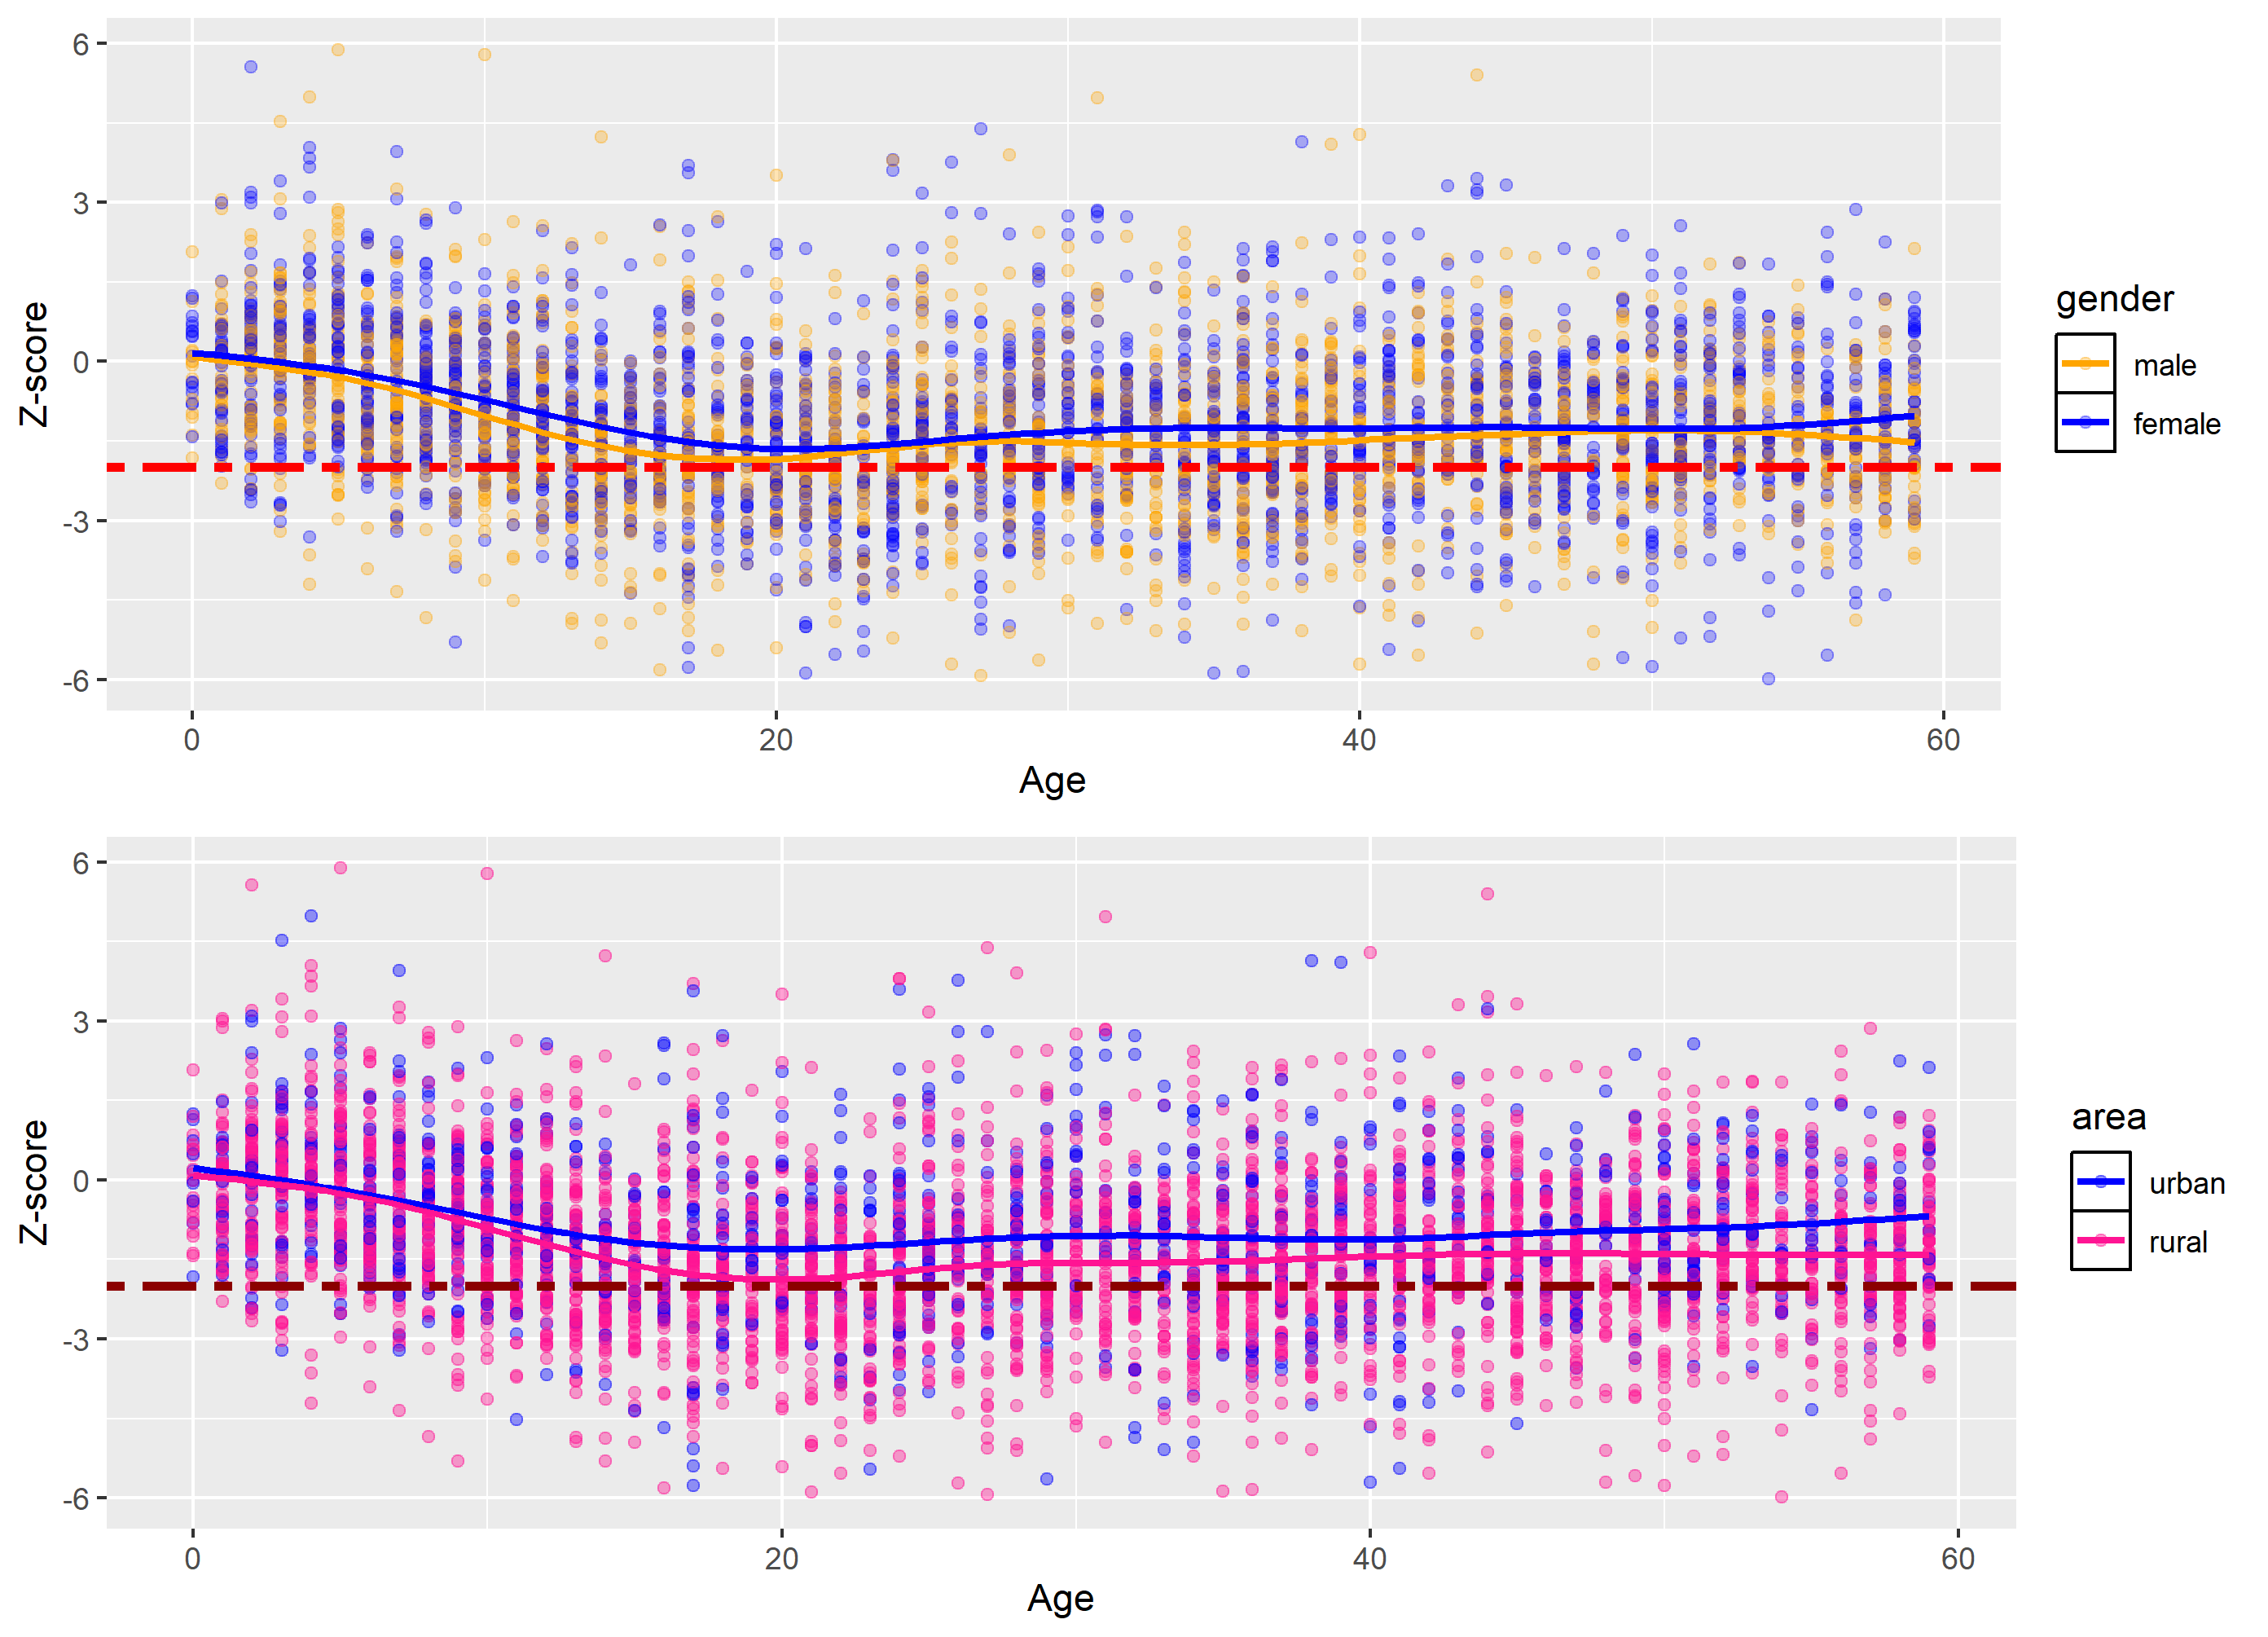
\includegraphics[scale=0.5]{ex1/scatter_1.png}
		\caption{Scatter plots  for age (in months) against Z-score split by gender (upper plot) and rural-urban factor (lower plot) with a smooth line. The red line (at \texttt{zstunt} $= - 2$) shows the critical value.}
		\label{fig:scatter_1}
\end{figure}

\newpage
\section{County wise Z-score}
In this exercise we use the functions of \texttt{tidyverse} and \texttt{ggplot2} to draw maps of counties. We take the data set provided by the GADM from the package \texttt{raster}. 
The task is to draw a map of Kenya's counties and fill the areas according to the mean Z-score (see Figure \ref{fig:kenya}). 

\begin{itemize}
    \item For the county Isiolo there is no data, so it's left gray
    \item As its represented in the legend, towards the shades of blue, more is Z-score and towards the shades of red, less is Z-score.
    \item There is visible differences in means Z-score between different counties
    \item We can observe a general pattern that the western and southern parts of the country suffers more from stunting than the northern parts.
    \item Except Kajiado all the counties in the south have a lower mean Z-score
    \item In the county West Pokot children are more stunted.
    \item Counties with good Z-score are on the boundaries in different direction. 
\end{itemize}
\begin{figure}[h]
    \centering
	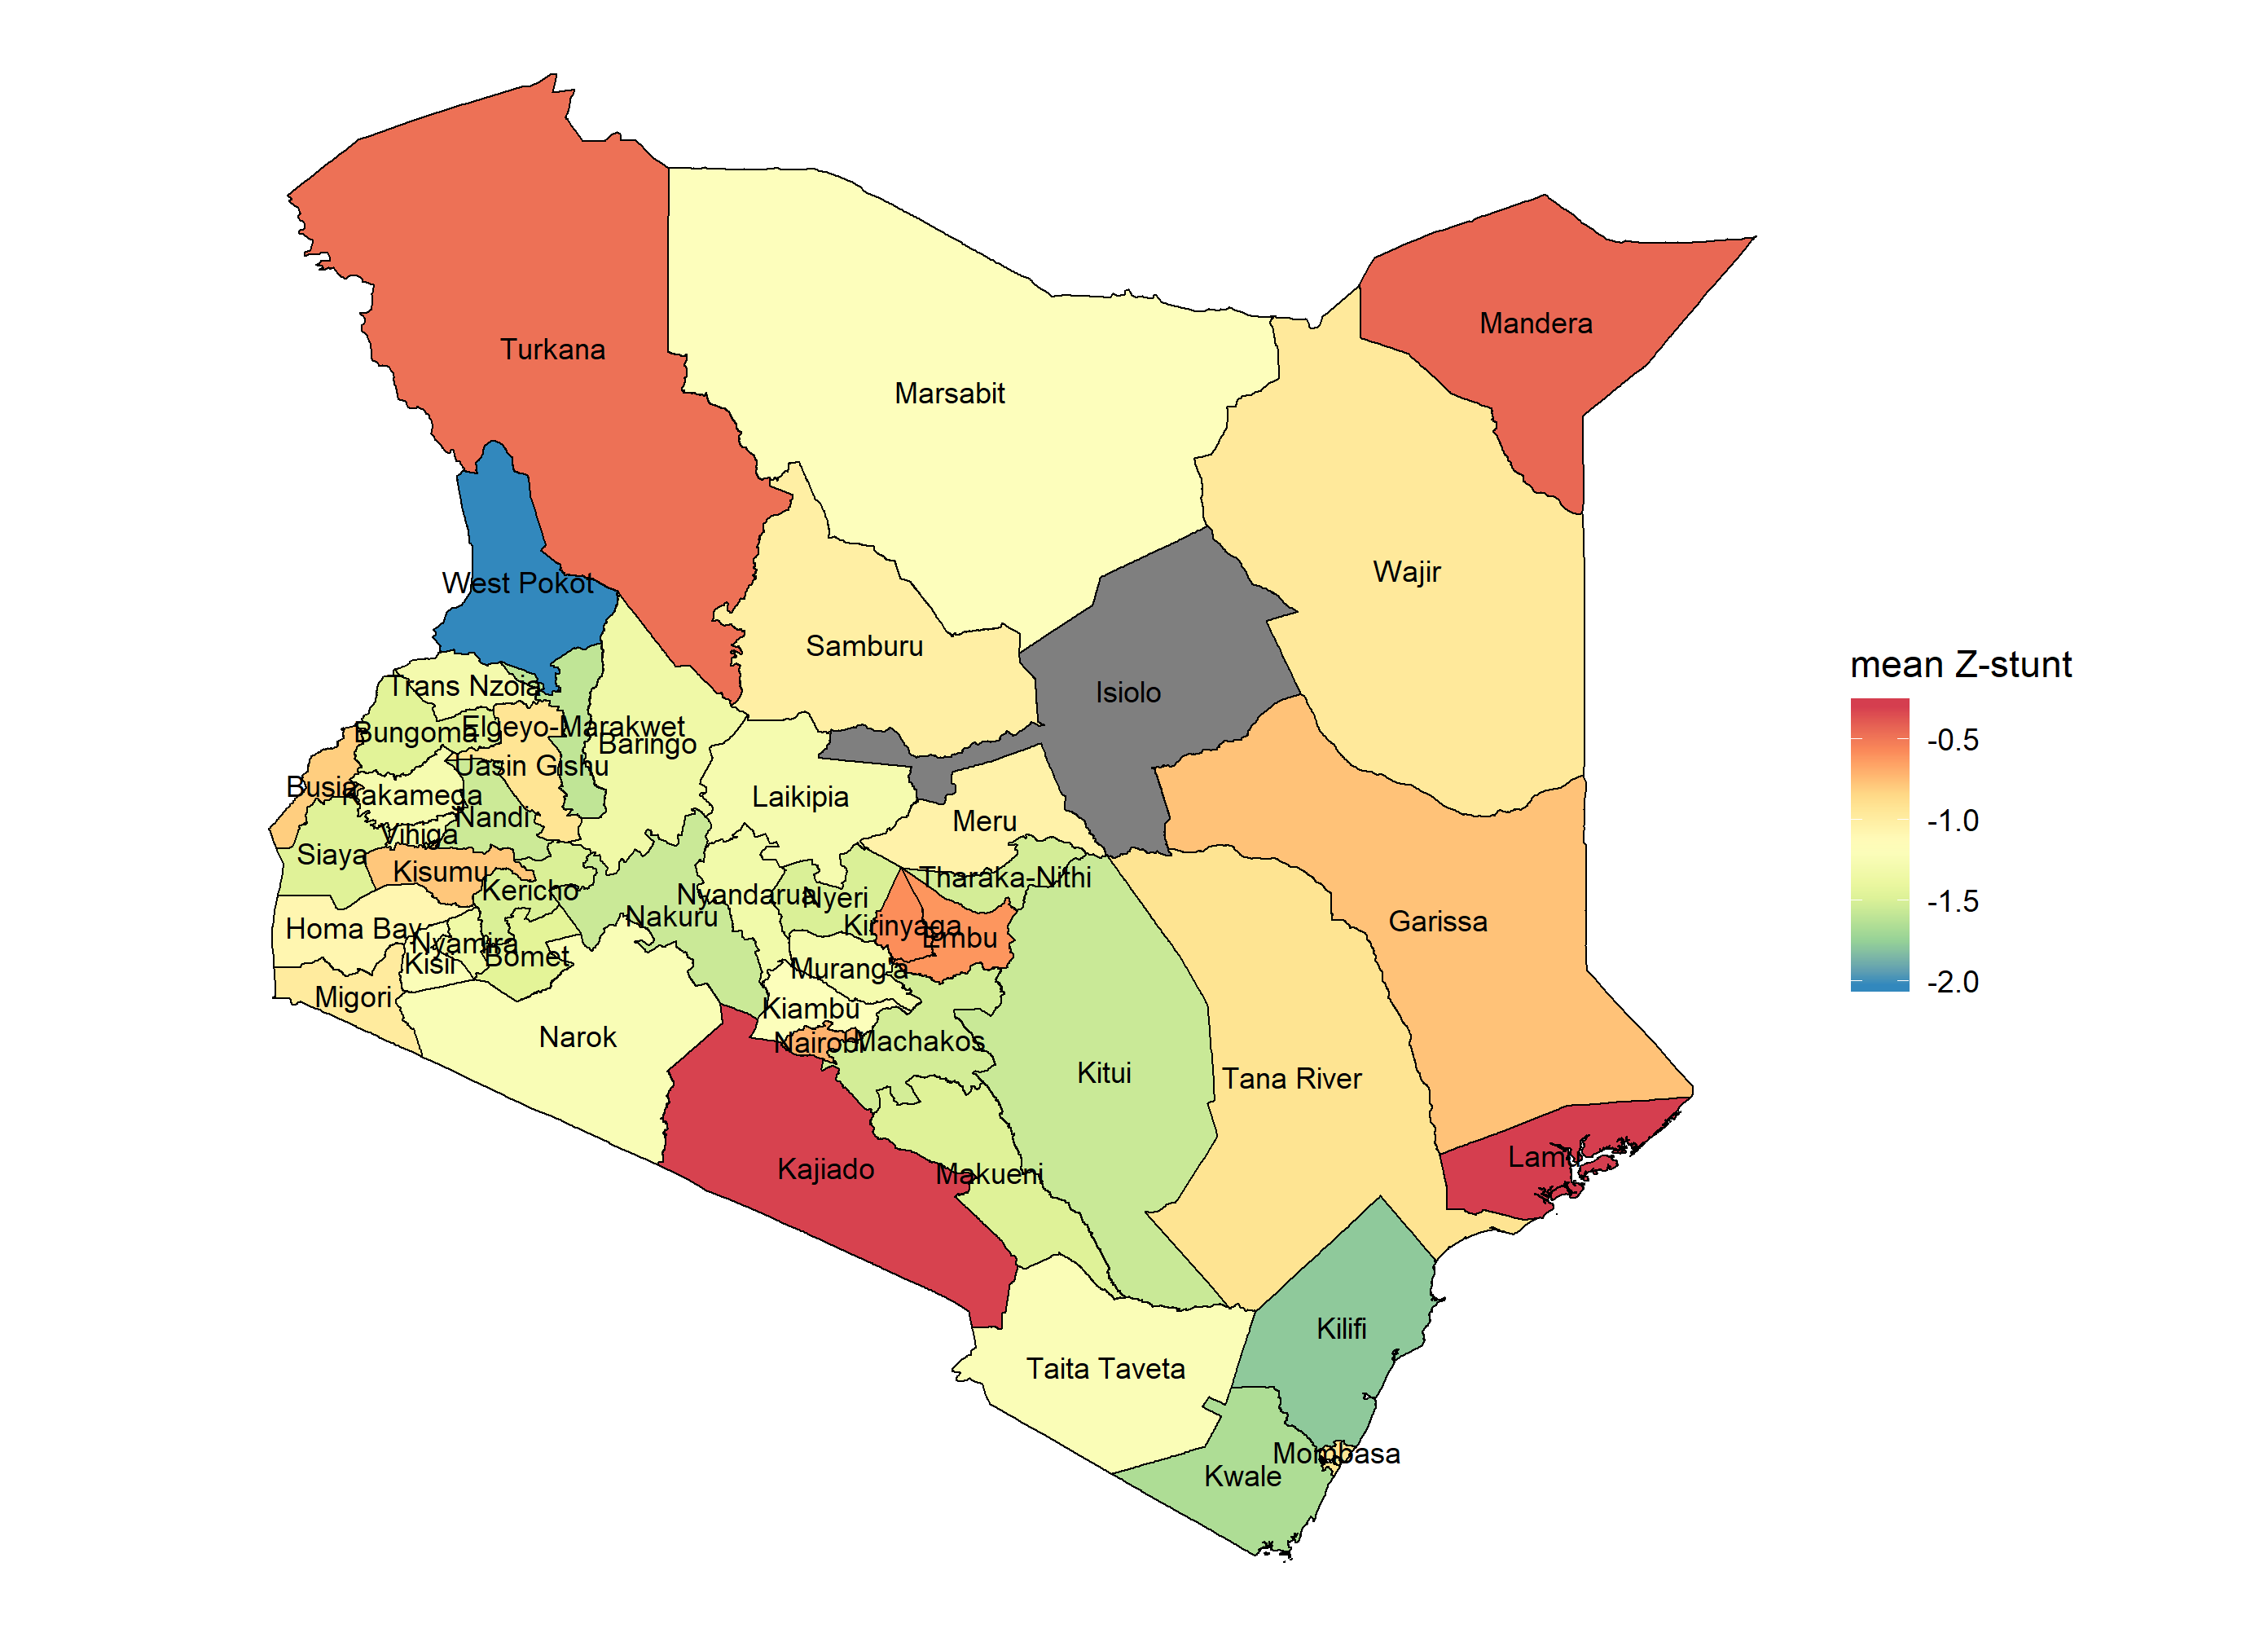
\includegraphics[scale=0.7]{ex1/Kenya.png}
	\caption{Map of Kenya with county-wise mean Z-score. }
	\label{fig:kenya}
\end{figure}
 